\chapter{Оригинальные результаты}

\section{Численное моделирование дифракционной решетки с переменным периодом.}

\subsection{Исследуемый образец}
В качестве исследуемой оптически неоднородной среды для метода когерентного контроля была выбрана дифракционная решетка в виду относительной простоты изготовления и изучения. Для непрерывного управления направлением распространения пучка была разработана трапециевидная форма щелей, такая, что при изменении относительной фазы двух когерентных источников эффективный период решетки непрерывно меняется за счёт сдвига пучности результирующей стоячей волны. В качестве материала был выбран аморфный кремний за его большой показатель преломления $n = 3,48$ и практически нулевой коэффициент поглощения для исследуемой длины волны $\lambda = 1550\ \text{нм}$. Для расчетов использовались табличные характеристики кремния, представленные на сайте\cite{refractiveIndex}. Полученная структура имеет множество геометрических параметров, а именно: периоды решетки и длины оснований трапеций на верхней и нижней границах $d_t$, $b_t$, $d_b$ и $b_b$ соответственно ($d_t < d_b$), число периодов $N$ и высота структуры $h$, указанные на Рис. \ref{fig:structure}А.

\begin{figure}
    \begin{center}
        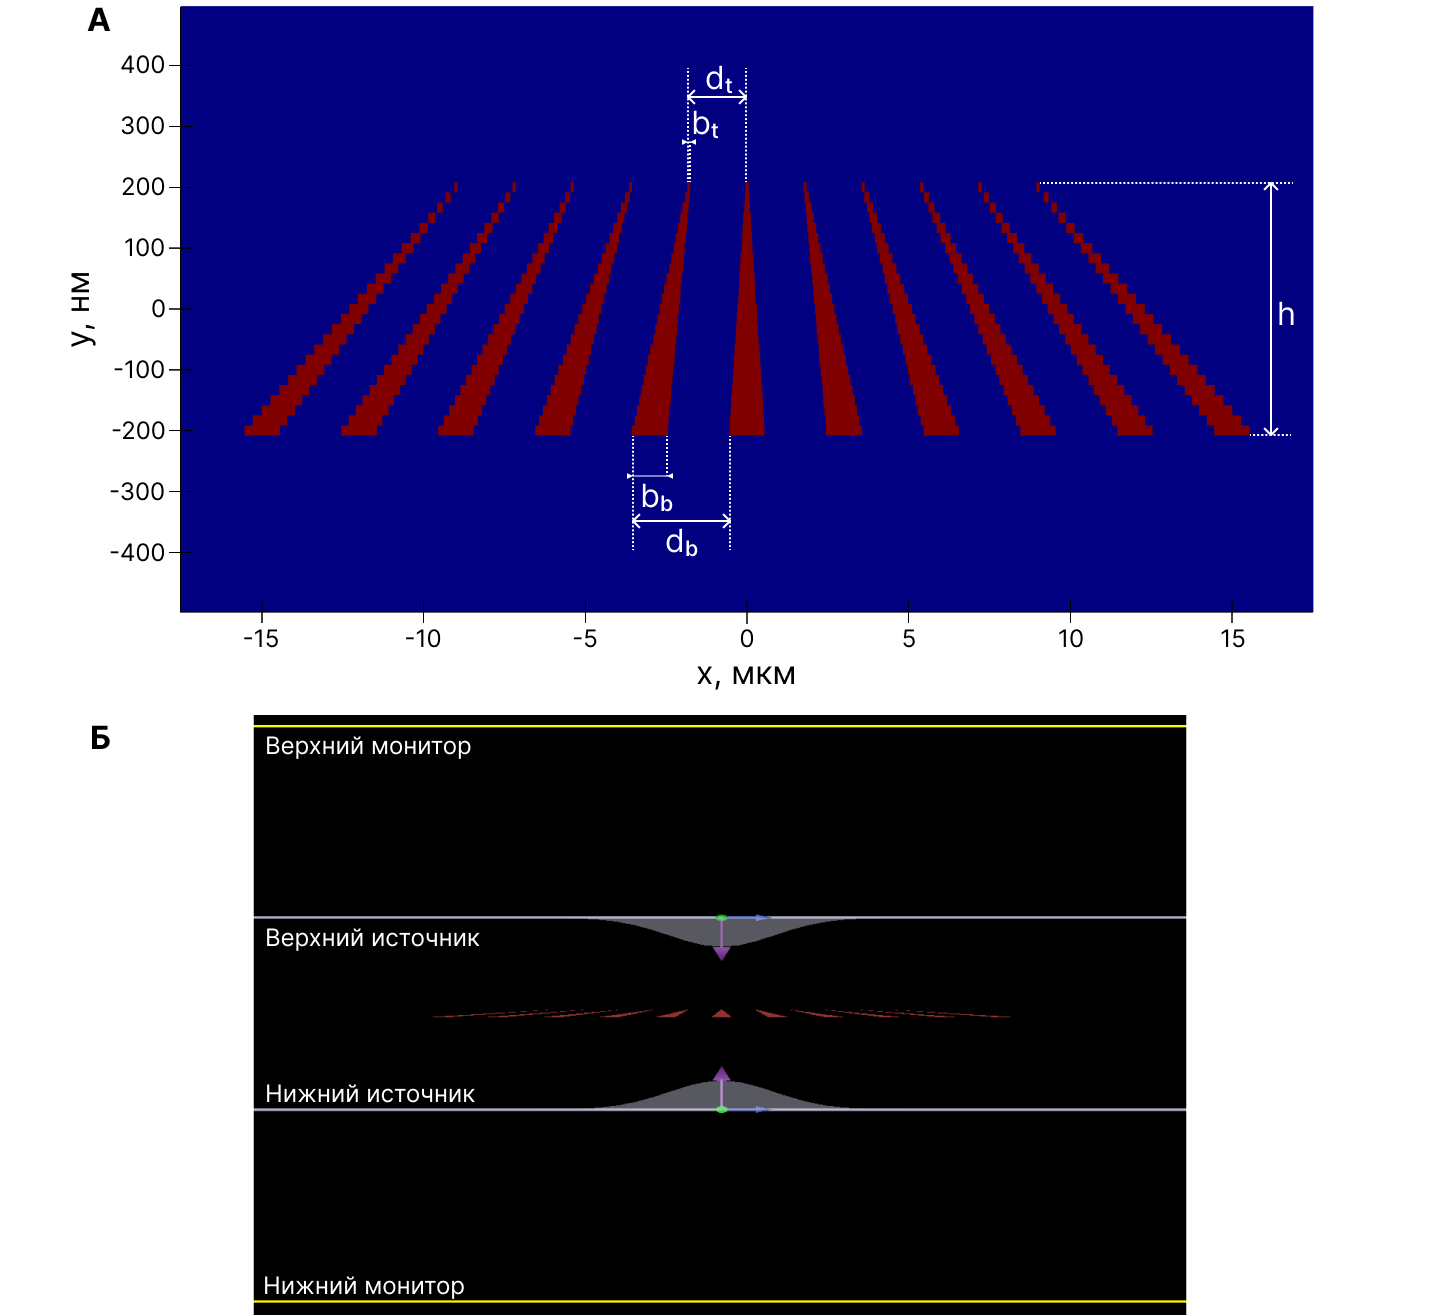
\includegraphics[width=\textwidth]{pictures/Structure.png}
        \caption{\textbf{(А)} Визуализация показателя преломления структуры с помощью монитора, представленного в пакете \texttt{Lumerical}. Параметры на рисунке: $d_t = 1800\ \text{нм}$, \mbox{$b_t = 300\ \text{нм }$}, $d_b = 3000\ \text{нм}$, $b_b = 1000\ \text{нм}$, $N = 11$, $h = 400\ \text{нм}$. Наблюдаемая <<лесенка>> связана с внутренним представлением области FDTD в программе. \textbf{(Б)}~Схема моделируемой системы.}
        \label{fig:structure}
    \end{center}
\end{figure}

\subsection{Программное обеспечение}
Основные результаты данной работы получены при помощи программного пакета \texttt{Ansys Lumerical FDTD} версии \texttt{2024 R1}, позволяющего моделировать поведение различных оптических систем. Его работа основана на численном методе конечных разностей во временной области (FDTD, англ. <<finite-difference time-domain>>). Характерные графики были построены на языке \texttt{Python} с помощью библиотек \texttt{numpy} и \texttt{matplotlib}. Результаты были структурированы и наглядно представлены с применением веб-технологий на языке \texttt{JavaScript}.

\subsection{Моделируемая система}
Схема моделируемой системы приведена на Рис. \ref{fig:structure}Б. На одинаковых расстояниях от структуры были расположены когерентные гауссовы источники с длиной волны $1550\ \text{нм}$ и длительностью импульса $10\ \text{фс}$. За ними находятся мониторы, которые выполняют Фурье-преобразование электрического поля и показывают профиль интенсивности дальнего поля. Радиус перетяжки $w = 5\ \text{мкм}$ был выбран так, чтобы задействовать максимальное число периодов решетки, но чтобы при этом дифракция на краях структуры была незначительной. Число периодов $10 \leqslant N \leqslant 15$ было ограничено из практических соображений сложности изготовления более протяженной решетки. Толщина $h \approx \lambda/4$ примерно равнялась четверти длины волны, чтобы на структуре при заданной разности фаз находилась только одна пучность, то есть имелся единственный эффективный период.

Время симуляции подбиралось таким образом, чтобы уровень энергии в системе к моменту окончания расчетов был достаточно низким, иначе полученные результаты могли бы оказаться неточными. Использовались граничные условия типа PML (англ. <<perfectly matched layer>>, <<идеально поглощающие слои>>), которые представляют собой поглощающую границу, моделирующую уход волны на бесконечность. Тем не менее, какая-то часть волн может отражаться от стенок и попадать обратно в область симуляции, приводя к искажениям. Шаг сетки, на которой программа выполняла численные расчеты, подбирался исходя из компромисса между временем симуляции и достаточным разрешением представления структуры.

\section{Расчет зависимости интенсивности излучения в первом дифракционном порядке от угла дифракции и сдвига фаз между источниками}

Исходя из качественных соображений и простейшего уравнения дифракционной решетки для нормального падения пучка:
\begin{equation}
    d\sin\Theta_m = m\lambda,
    \label{eq:simpleGrating}
\end{equation}
были ограничены $d_t$ и $d_b$ решетки так, чтобы наблюдался только первый порядок дифракции:
\begin{equation}
    d_{min} = \lambda = 1550\ \text{нм},\ d_{max} = 2\lambda = 3100\ \text{нм}.
\end{equation}
Приблизительно в данных пределах фиксировались определенные значения $d_t$ и $d_b$, связанные с углом обзора соотношением
\begin{equation}
    \mathrm{FOV} = \Theta_{max} - \Theta_{min} = \arcsin{\frac{\lambda}{d_t}} - \arcsin{\frac{\lambda}{d_b}},
    \label{eq:fov}
\end{equation}
и циклично запускалась симуляция, на каждом шаге которой последовательно изменялись $b_t$ и $b_b$ в пределах 100--1500 нм и сохранялись результаты вычислений с обоих мониторов. Таким образом, для каждой пары $d_t$--$d_b$ было получено \mbox{$15 \cdot 15 \cdot 2 = 450$} наборов данных, по которым затем строились графики зависимости интенсивности излучения в первом дифракционном порядке от угла дифракции и сдвига фаз между источниками типа <<тепловая карта>>.

\begin{figure}
    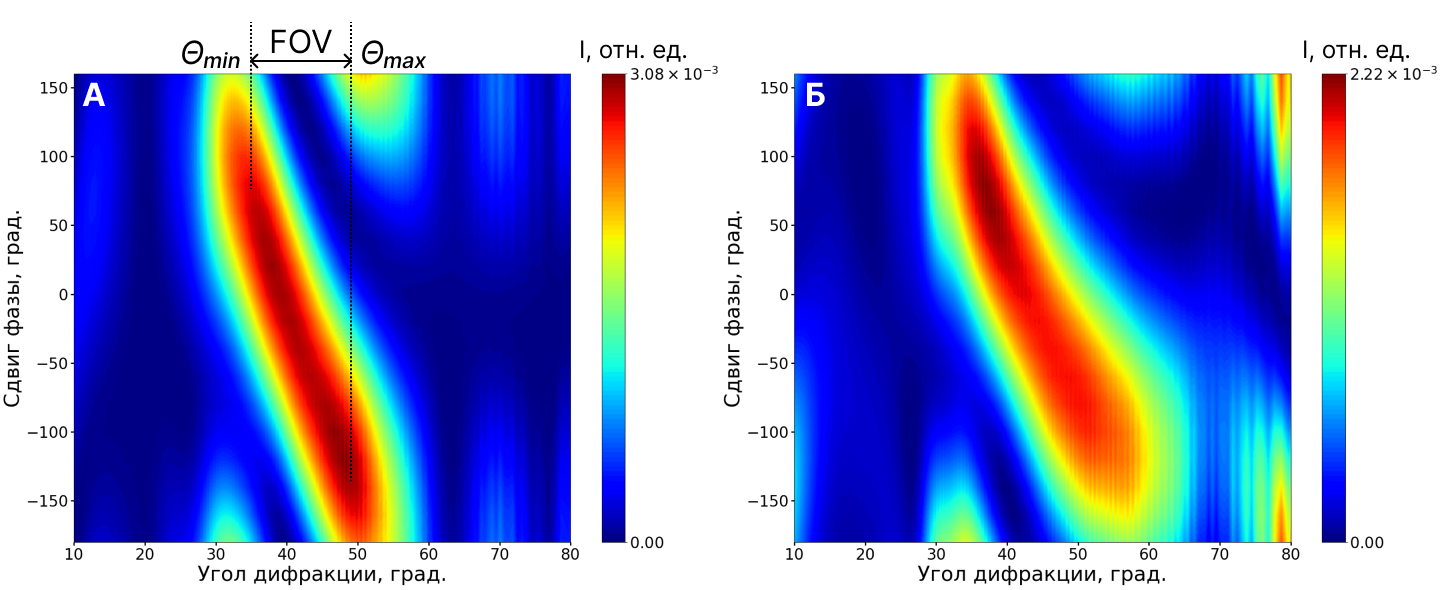
\includegraphics[width=\textwidth]{pictures/Heatmaps.png}
    \caption{Избранные графики зависимости интенсивности излучения в первом дифракционном порядке от угла дифракции и сдвига фаз между источниками. \textbf{(А)} Полученная конфигурация с углом обзора 15°: $N = 11$, $d_t = 1800$~нм, $d_b = 3000$~нм, $b_t = 1100$~нм, $b_b = 500$~нм. \textbf{(Б)} Полученная конфигурация с углом обзора 20°: $N = 15$, $d_t = 1550$~нм, $d_b = 3100$~нм, $b_t = 1100$~нм, $b_b = 400$~нм. }
\end{figure}

\section{Результаты}

Все полученные графики представлены на \href{https://fizfakovets.github.io}{\underline{сайте}}. Были найдены конфигурации, позволяющие осуществлять непрерывный контроль распространения пучка в диапазоне 35--55°. В результате оптимизации значений $b_t$ и $b_b$ удалось достичь равномерной интенсивности дифракционного порядка при изменении фазы одного из источников. В рамки настоящей работы не входило достижение высокого разрешения сканирования, поэтому на графике можно видеть большую угловую расходимость пучка. Однако это можно исправить, направляя на решетку более коллимированное излучение.
